\chapter{Chapter 5: Results and Analysis}

Analogous expressions apply for Y and Z. The pipeline results reported in Chapter 5 use the corrected model. It should be noted that the bias and scale parameters were estimated from the same 36-point static ball dataset used for final accuracy reporting; an independent held-out calibration set was not used. The correction therefore reflects in-sample fitting, and the reported corrected errors may underestimate the true generalisation error. This limitation should be considered when interpreting the corrected accuracy figures.

\section{Intrinsic Calibration Results}

Intrinsic calibration was performed at 1280 \(\times\) 720 resolution for all four cameras using the ChArUco auto-capture procedure. Subsequently 30--40 valid frames per camera were collected to achieve stable parameter estimates.

Per-camera reprojection errors after calibration are in the range of 2--8 pixels between the four cameras which is acceptable for this application. The difference between cameras is due to the quality of the lenses and the spatial distribution of captured calibration poses. CamSouth, located furthest from the area normally calibrated, had the highest reprojection error of this range, and took 2 captures to get a valid calibration frame set.

The resulting K matrices confirm focal lengths in the expected range for a 1280-pixel-wide sensor with a moderately wide field of view, and distortion coefficients consistent with a barrel distortion pattern typical of low-cost webcam lenses. Undistortion is applied to all frames before detection inference and before triangulation.

\section{Extrinsic Calibration Results}

Extrinsic calibration using the 24-AprilTag wall grid produced camera poses with residual reprojection errors of 3--7 pixels after robust outlier rejection. On average, sigma-scale = 2.0 outlier rejection removed 8--15\% of tag corner observations, primarily from tags at oblique angles near the arena edges where detection reliability decreases.

The overlay validation procedure (reprojecting known AprilTag corner positions back into each camera frame and comparing with detected positions) confirmed visual alignment across all four cameras. In all cameras, reprojected corners fell within 5--10 pixels of detected corners across the majority of the visible tags.

The resulting world-frame camera positions (Table~\ref{tab:3_1}) are consistent with physical tape measurements of the mounted camera positions to within approximately \(\pm\)30 mm, confirming the calibration is geometrically reasonable.

\section{Ball Static Localisation Results}

\begin{table}[htbp]
\centering
\caption{Ball static localisation summary metrics (corrected pipeline)}
\label{tab:5_1}
\begin{tabular}{|l|l|}
\hline
\textbf{Metric} & \textbf{Value} \\
\hline
Trials valid & 36 / 36 (100\%) \\
\hline
Mean 3D error & 95.17 mm \\
\hline
Median 3D error & 84.18 mm \\
\hline
RMSE & 102.23 mm \\
\hline
P90 & 142.18 mm \\
\hline
P95 & 166.51 mm \\
\hline
Maximum error & 214.60 mm \\
\hline
Mean reprojection error & 6.01 px \\
\hline
Mean cameras used & 2.87 \\
\hline
Mean detection ratio (hold window) & 1.000 \\
\hline
Mean temporal precision (std over hold) & 3.79 mm \\
\hline
P95 temporal precision & 8.51 mm \\
\hline
\end{tabular}
\end{table}

The uncorrected pipeline exhibited systematic biases: X-axis bias of +50.68 mm (estimated positions shifted toward higher X), Y-axis bias of +46.57 mm (estimated positions shifted toward higher Y), and Z-axis bias of \textminus{}106.98 mm (estimated positions systematically below true height).

The Z-axis bias is the dominant systematic error. It is attributed primarily to the camera mounting heights: all four cameras are mounted near the ceiling, which means that they see the ball from above. Triangulation of a ball at low Z (200--700 mm from the floor) consists of shallow downward looking ray angles, which are geometrically sensitive to small calibration errors of the extrinsic Z positions of the cameras. The negative Z bias is consistent with the fact that the cameras have been calibrated as a bit lower than their true physical height causing triangulated points to be placed below their true elevation.

After the application of the linear axis correction model the mean error decreases from approx. 150.77 mm (raw) to 95.17 mm (corrected) and the P95 from approx. 288.34 mm to 166.51 mm. Both of the main acceptance criteria (mean < 120 mm, P95 < 200 mm) are met by the corrected pipeline.

Temporal precision, defined as the standard deviation of repeated estimates of the same static point over the hold window, averages 3.79 mm with a P95 of 8.51 mm. This demonstrates that the triangulation pipeline is highly repeatable given consistent input observations; the dominant error source is systematic calibration bias rather than random noise.

\begin{figure}[htbp]
\centering
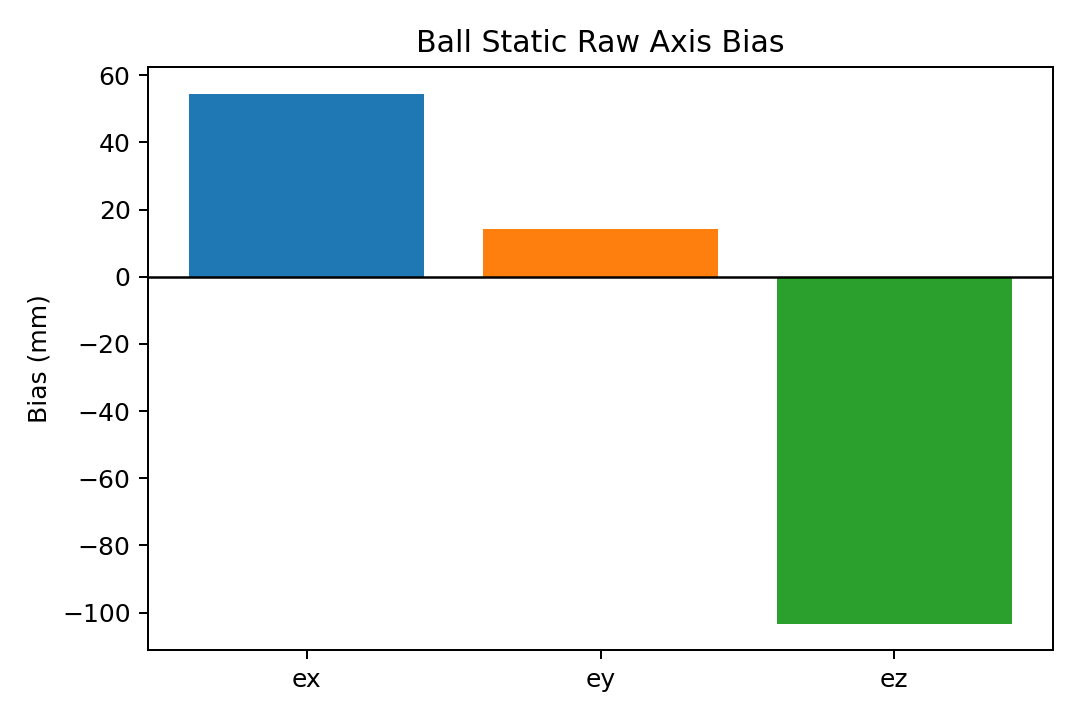
\includegraphics[width=0.8\textwidth]{figures/image5_2_raw_vs_corrected}
\caption{Ball static localisation: raw vs corrected 3D error comparison, demonstrating the linear bias correction model reducing mean error from 150.77 mm to 95.17 mm.}
\label{fig:5_2}
\end{figure}

\begin{figure}[htbp]
\centering
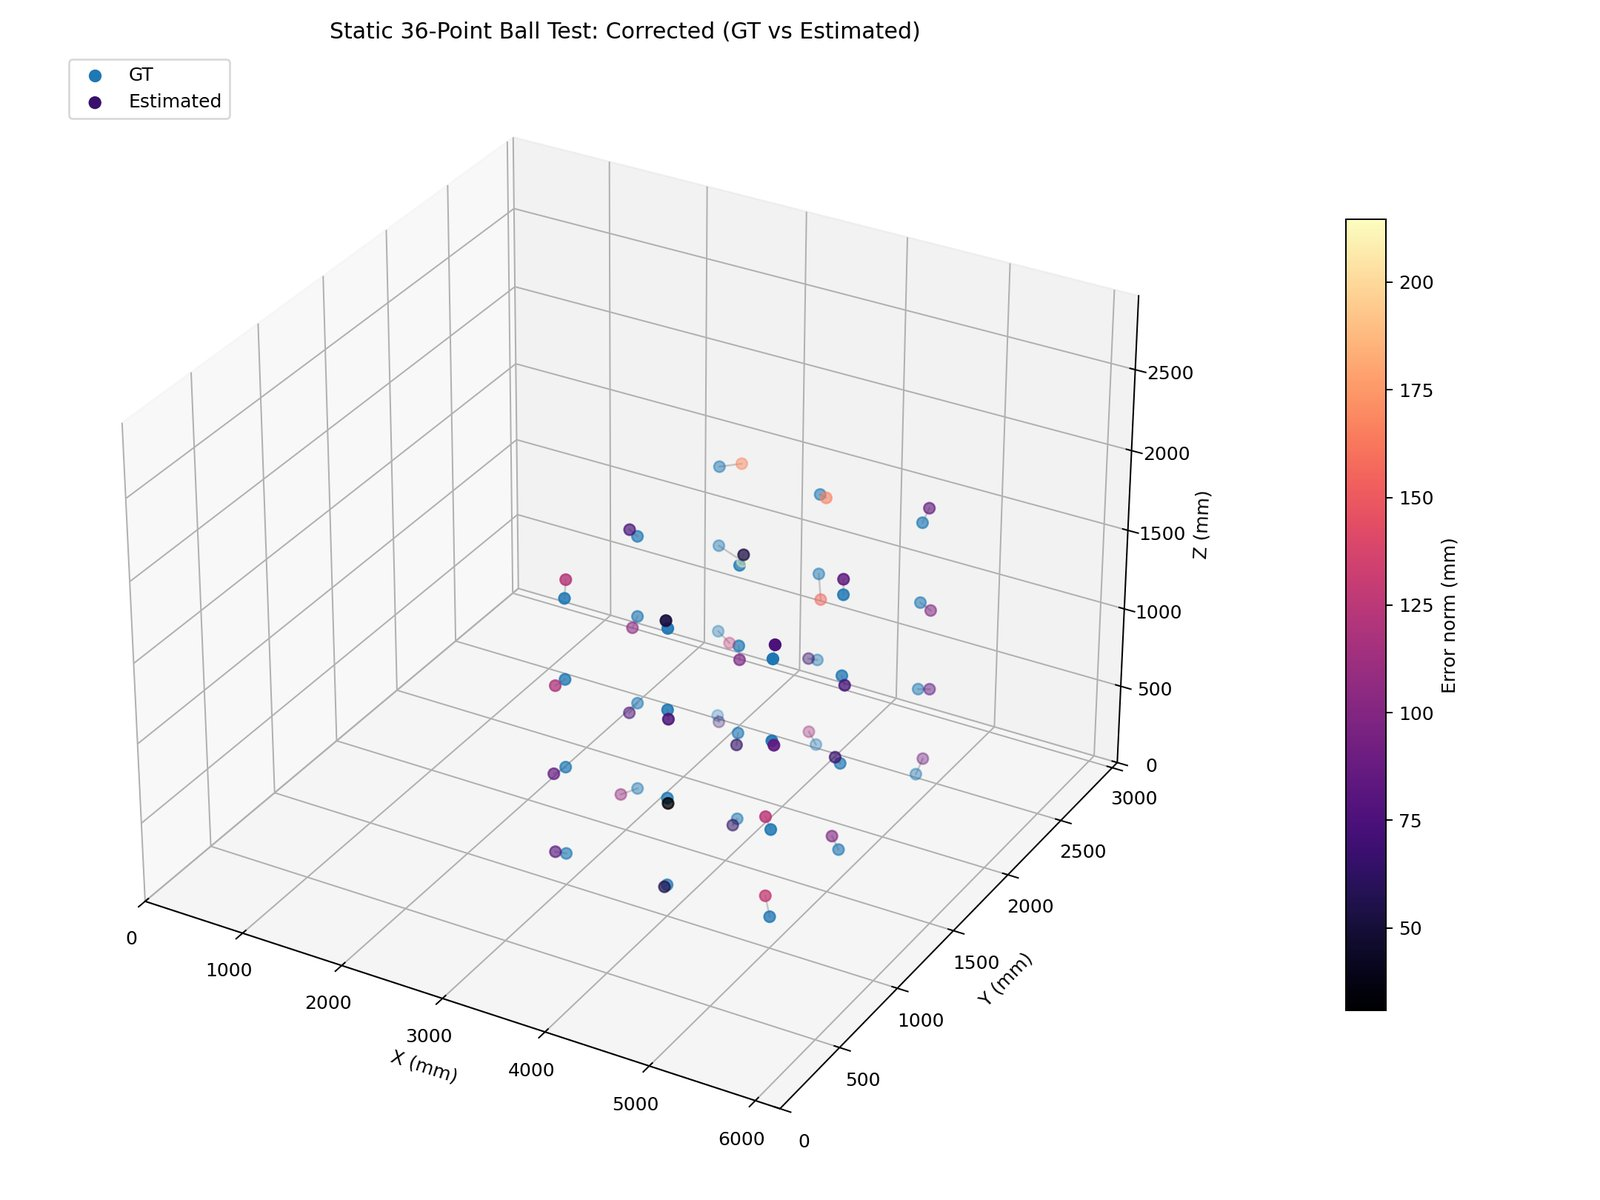
\includegraphics[width=0.8\textwidth]{figures/image5_3_3d_scatter}
\caption{3D scatter of ground-truth (blue) vs corrected estimated (coloured by error magnitude) ball positions across all 36 trials. The colour bar indicates error norm in mm.}
\label{fig:5_3}
\end{figure}

A spatial overview of the entire 36-point static evaluation grid is given in Figure~\ref{fig:5_3}. These ground-truth positions (blue) are associated with its corrected estimate, coloured according to its error magnitude. The greatest errors (warm colours, 150--215 mm) are centred around the corners of the arena and at the highest layer of the Z (1800 mm) where the cameras see the ball at near-vertical angles and the geometry for triangulation is weakest. Low to moderate errors (cool colours, <100 mm) dominate the mid-height layers (750--1300 mm), confirming that the correction model is most effective in the central working volume of the arena.

\begin{figure}[htbp]
\centering
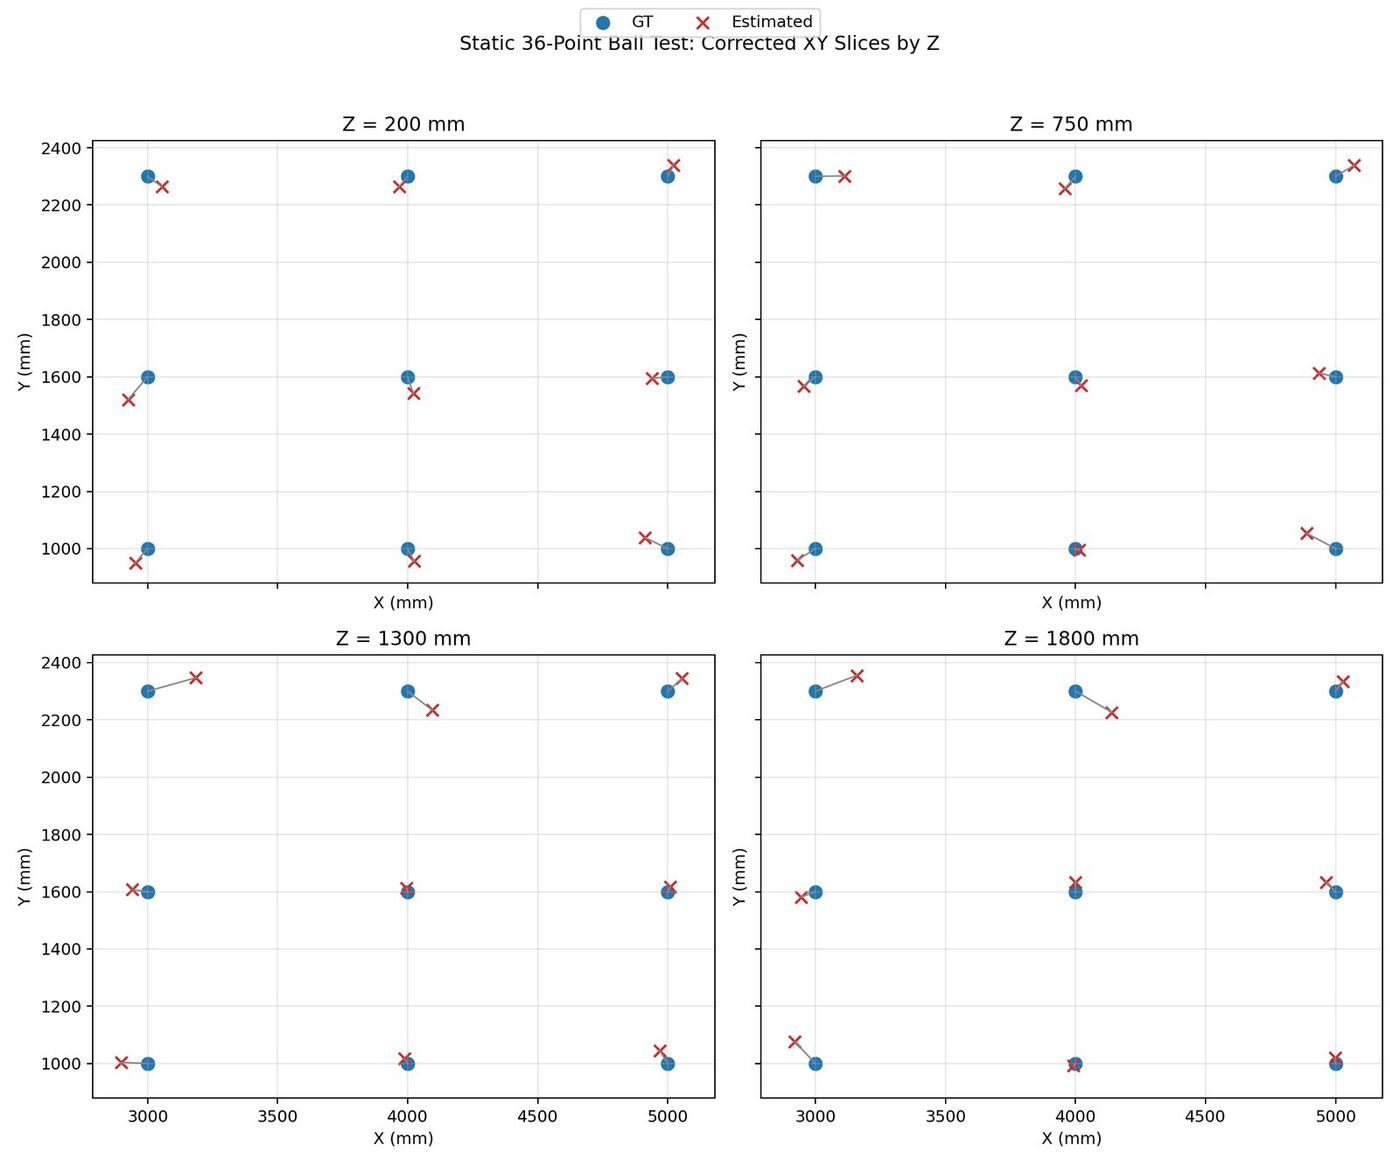
\includegraphics[width=0.8\textwidth]{figures/image5_4_xy_slices}
\caption{XY-plane slices at four Z heights (200, 750, 1300, 1800 mm) showing ground-truth (blue circles) vs corrected estimates (red crosses).}
\label{fig:5_4}
\end{figure}

The slice view in Figure~\ref{fig:5_4} isolates each height layer, making the spatial distribution of errors easier to interpret. At Z = 200 mm and Z = 750 mm, the corrected estimates closely track the ground-truth grid, with small and consistent offsets. At Z = 1300 mm, a slight drift in the X direction becomes visible at the far end of the arena (X \(\approx\) 5000 mm). At Z = 1800 mm, the offsets are largest and least uniform, reflecting the diminished triangulation baseline that results from all cameras being mounted near the ceiling.

\section{Human Pose Joint-Touch Results}

\begin{table}[htbp]
\centering
\caption{Joint-touch 3D ground-truth summary metrics (62 valid trials)}
\label{tab:5_2}
\begin{tabular}{|l|l|}
\hline
\textbf{Metric} & \textbf{Value} \\
\hline
Trials valid & 62 / 81 (76.5\%) \\
\hline
Mean 3D error & 143.38 mm \\
\hline
Median 3D error & 148.90 mm \\
\hline
RMSE & 147.73 mm \\
\hline
P90 & 182.04 mm \\
\hline
P95 & 198.73 mm \\
\hline
Maximum error & 217.34 mm \\
\hline
\end{tabular}
\end{table}

\begin{table}[htbp]
\centering
\caption{Per-joint error breakdown}
\label{tab:5_3}
\begin{tabular}{|l|l|l|}
\hline
\textbf{Joint} & \textbf{Mean error (mm)} & \textbf{P95 (mm)} \\
\hline
right\_knee & 110.03 & 170.75 \\
\hline
right\_hip & 150.38 & 172.31 \\
\hline
left\_shoulder & 164.38 & 199.54 \\
\hline
\end{tabular}
\end{table}

The right knee achieves the lowest mean error (110.03 mm), consistent with its position at mid-height where all four cameras have favourable viewing geometry. The right hip is observed at a greater height and can be partially occluded by the subject's torso from lateral cameras, resulting in higher error (150.38 mm). The left shoulder, at the greatest height (1560--2200 mm depending on platform level), is closest to the ceiling camera mounting positions and therefore observed at increasingly oblique angles; additionally, the left shoulder is the joint most likely to be occluded by the subject's head and neck. This produces the highest mean error (164.38 mm).

The global P95 of 198.73 mm is below the acceptance threshold of 280 mm, and the per-joint P95 values (170.75, 172.31, 199.54 mm) are all below the per-joint thresholds (220, 220, 250 mm respectively). The mean error of 143.38 mm is below the acceptance threshold of 180 mm.

The 19 invalid trials (23.5\% of 81) represent a limitation of the evaluation methodology. In most invalid cases, the subject's body occluded the target joint from one or more cameras during the hold, reducing the camera count below the minimum threshold. This is a real operational constraint: the system requires at least three cameras with clear joint visibility for accurate 3D joint localisation.

\begin{figure}[htbp]
\centering
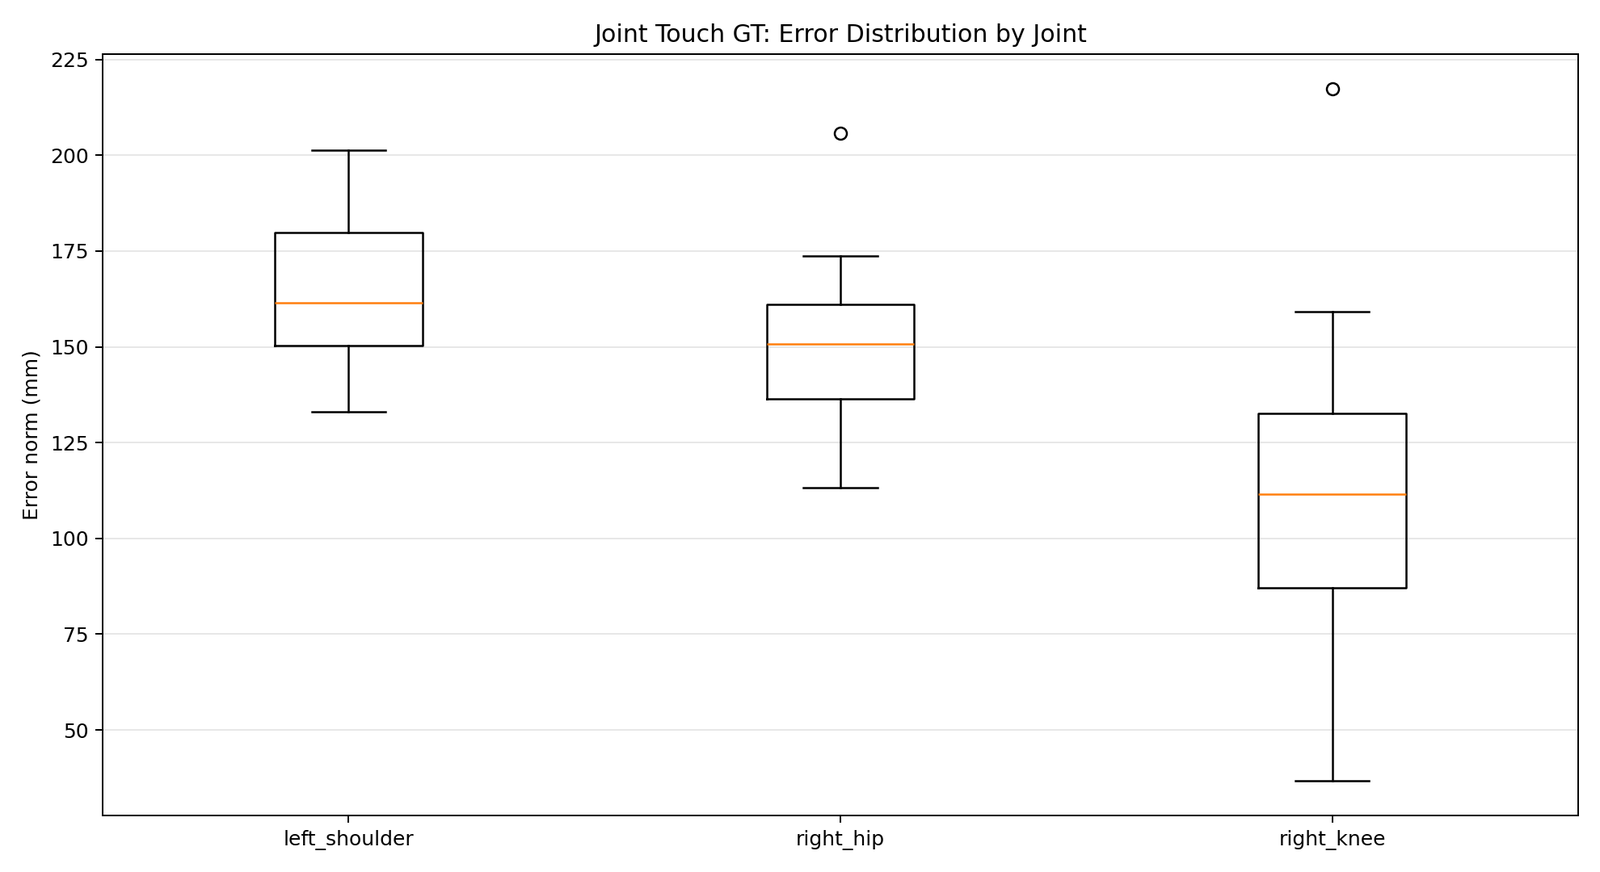
\includegraphics[width=0.8\textwidth]{figures/image5_5_joint_boxplot}
\caption{Joint-touch 3D error boxplot by joint type, showing right\_knee (110.03 mm mean), right\_hip (150.38 mm), and left\_shoulder (164.38 mm).}
\label{fig:5_5}
\end{figure}

The box plot in Figure~\ref{fig:5_5} agrees with the error hierarchy per joint quantitatively. The right\_knee has the lowest median error (111.5 mm), and the widest error in the spread (IQR \(\approx\) 45 mm), including one outlier above 217 mm. The right\_hip depicts a tighter distribution (IQR \(\approx\) 20 mm) with a median of 150.7 mm suggesting better consistency of error but higher errors. The left\_shoulder has the greatest median (161.6 mm) and a narrow IQR, indicating that the Z-axis bias has uniform effect on this high joint. Two outliers close to 205 mm (right\_hip) and 217 mm (right\_knee) are trials in which the mannequin was placed at the arena boundary, where less than three cameras were able to track the target joint.

\begin{figure}[htbp]
\centering
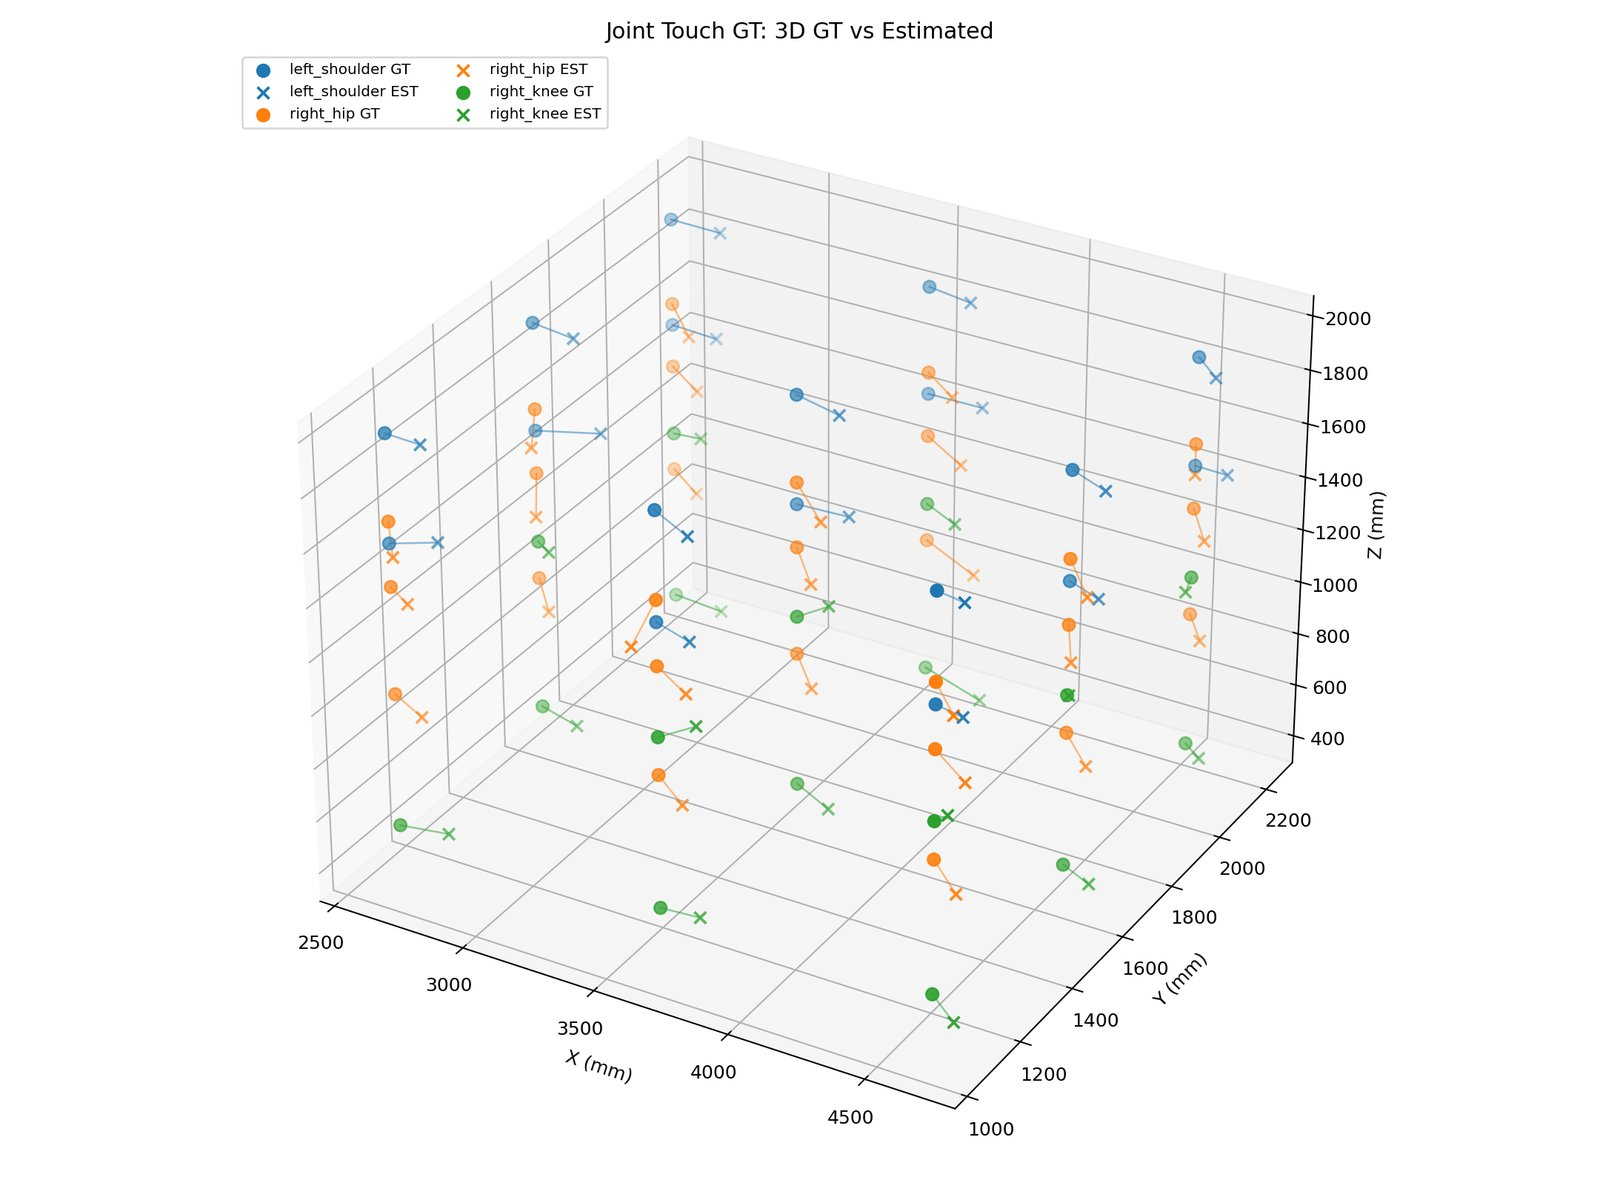
\includegraphics[width=0.8\textwidth]{figures/image5_6_joint_3d}
\caption{Joint-touch ground-truth vs estimated positions: 3D scatter plot showing all 62 valid trials with GT markers and estimated positions colour-coded by joint type.}
\label{fig:5_6}
\end{figure}

Figure~\ref{fig:5_6} visualises the spatial correspondence between ground-truth and estimated joint positions in the full volume of the arena. The connecting lines between GT and EST pairs highlight consistent directional offset between estimates with left\_shoulder estimates in blue setting an offset of -118 mm in Z and right\_knee estimates in green having the smallest mean displacement of 110 mm for the whole. The estimates from the right\_hip (orange) have a tight clustering in mid-volume with spatially uniform error. This joint-dependent pattern is consistent with the varying visibility by the camera at different body heights, with lower joints (knee) being more reliably triangulated, because they are in the strongest part of the camera overlap zone.

\begin{figure}[htbp]
\centering
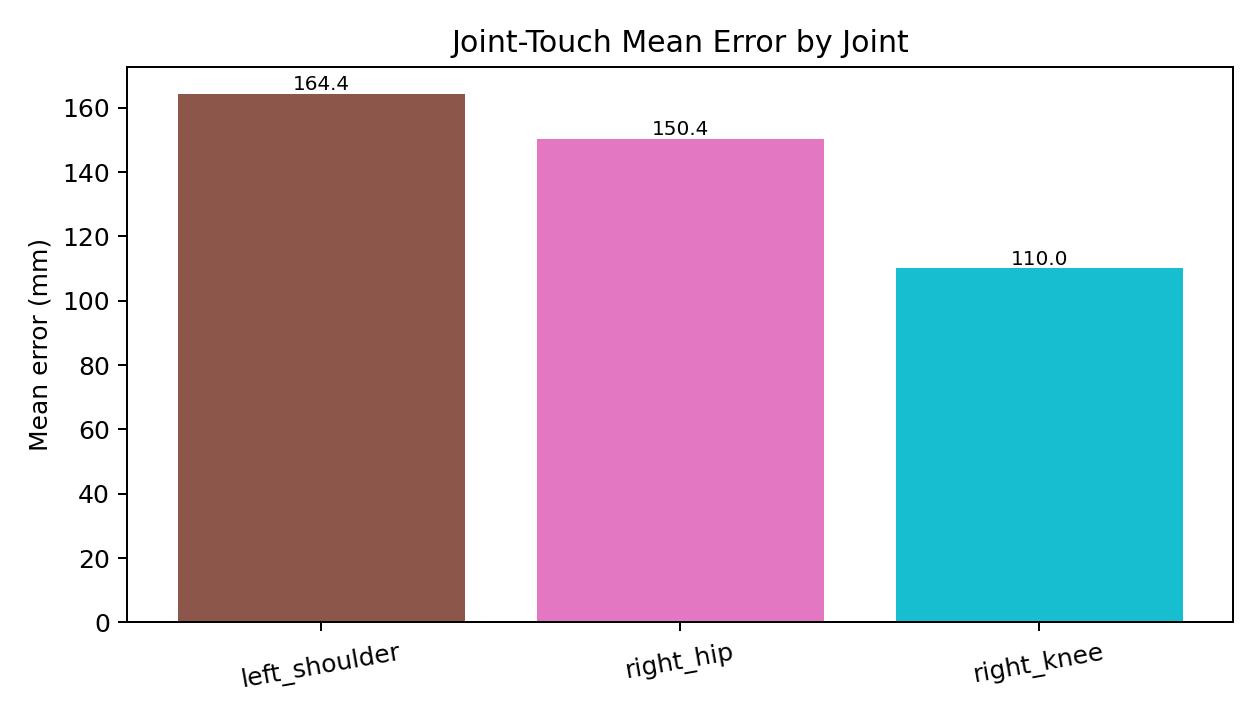
\includegraphics[width=0.8\textwidth]{figures/image5_8_joint_scatter}
\caption{Mean 3D error by joint type: bar chart confirming the monotonic increase in error from knee to shoulder, consistent with decreasing camera visibility at greater heights.}
\label{fig:5_7}
\end{figure}

Figure~\ref{fig:5_7} summarises the per-joint mean errors as a bar chart: left\_shoulder 164.4 mm, right\_hip 150.4 mm and right\_knee 110.0 mm. The monotonic decrease in shoulder to knee is coherent with the decreasing camera visibility with height of the body discussed in Section 5.4.

\section{Dynamic Detection Results}

\begin{figure}[htbp]
\centering
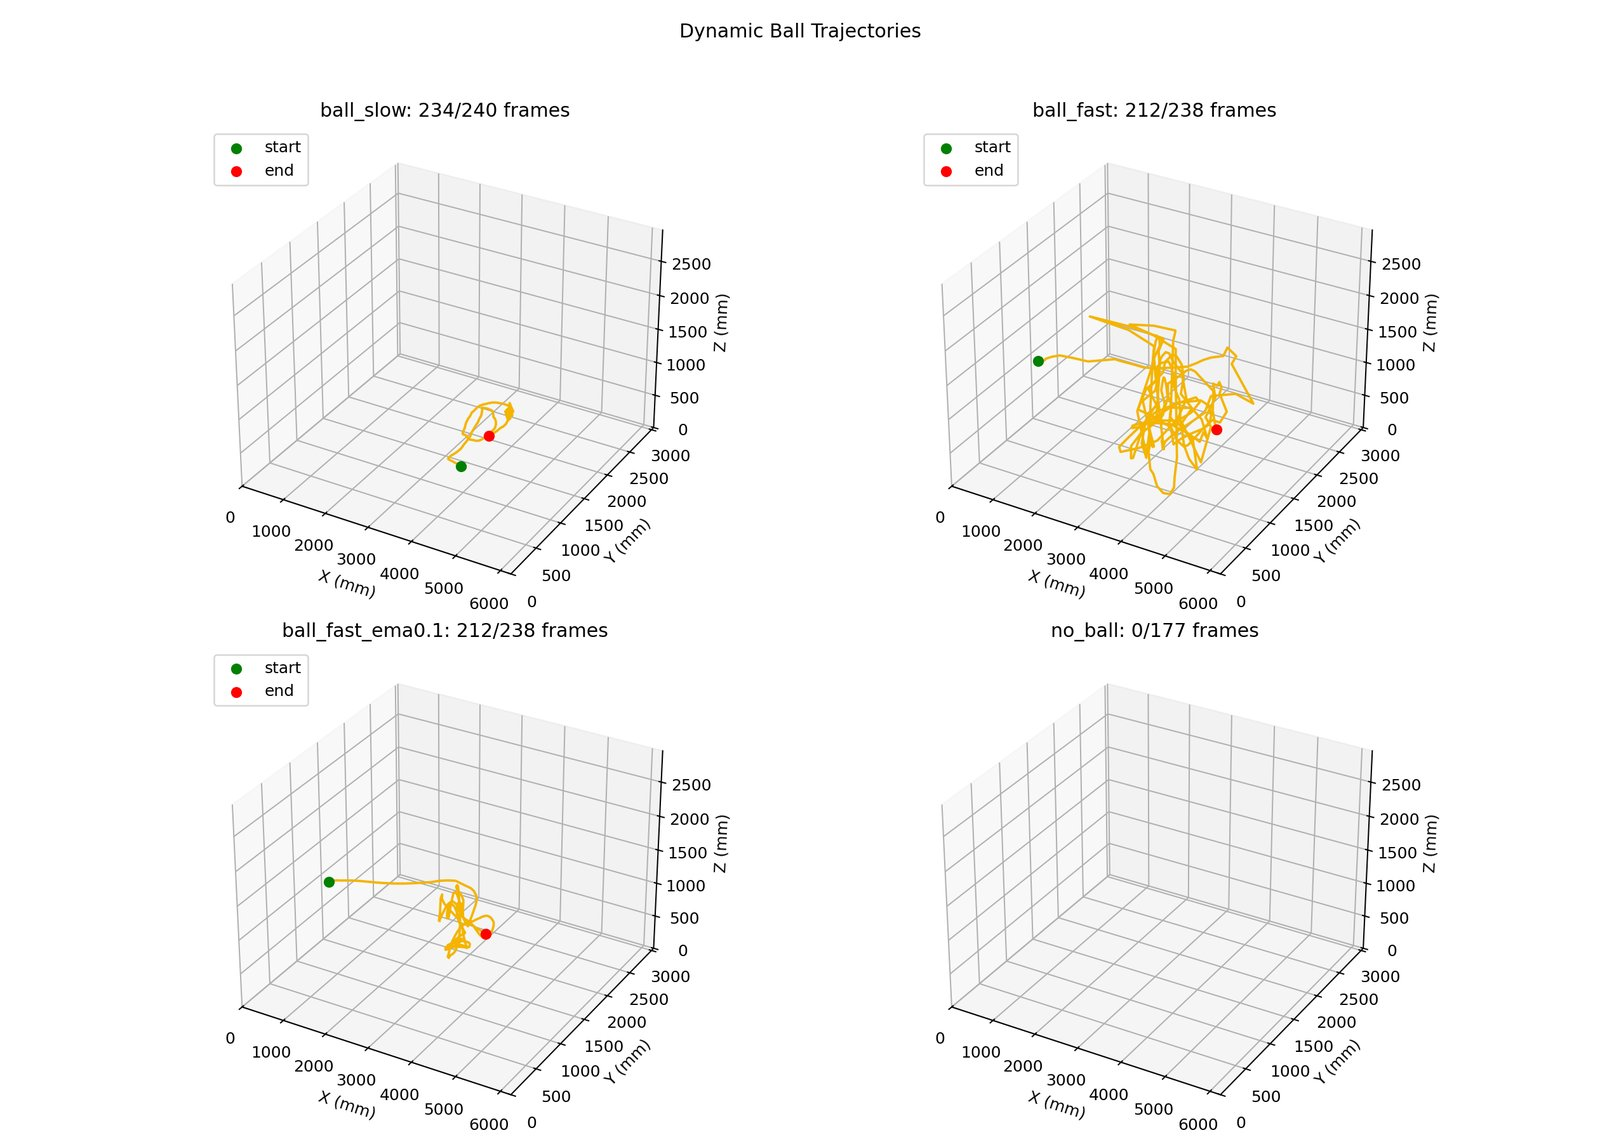
\includegraphics[width=0.8\textwidth]{figures/image5_9_dynamic}
\caption{Dynamic ball trajectory reconstructions: 3D plots of the four validation clips (\textit{ball\_slow}, \textit{ball\_fast}, \textit{ball\_fast\_ema0.1}, and \textit{no\_ball}) showing start (green) and end (red) markers.}
\label{fig:5_8}
\end{figure}

The 3D trajectory reconstructions for all 4 dynamic validation clips are shown in Figure~\ref{fig:5_8}. There were no jumps in the 3D reconstruction at all: the \textit{ball\_slow} clip ran for 20 seconds with no frame-to-frame jumps measured over 800 mm. The EMA filter was able to suppress minor jitter without lag being noticeable. In the \textit{ball\_fast} clip, the trajectory is more erratic, which is to be expected in the situation of higher ball speeds where their motion blur restricts their detection confidence. A stronger EMA smoothing application ($\alpha = 0.1$) in \textit{ball\_fast\_ema0.1} effectively tightens the trajectory at the expense of a small lag. The \textit{no\_ball} control clip correctly produced no sustained trajectory, confirming the detector does not hallucinate ball positions when no ball is present. These results confirm the pipeline is suitable for tracking moving targets at moderate speeds in the arena.

